\RequirePackage[T1]{fontenc}
\documentclass[conference,letterpaper]{IEEEtran}
\usepackage{cite}
\usepackage{amsmath,amssymb,booktabs,graphicx}
\usepackage[hidelinks]{hyperref}
\urlstyle{same}
\title{Output-Column Reuse in a Coherent GEMM Accelerator:
Tile Width and Memory-System Effects}
\author{\IEEEauthorblockN{Yasir Mahmud, Rasin Mohammed Ihtemam, and Mohyeu Hussain}
\IEEEauthorblockA{EEL 5764: Computer Architecture\\Fall 2026}}
% Generated by scripts/build_paper_numbers.py from paper/experiment_data.json.
\newcommand{\SpeedupEight}{0.875}
\newcommand{\ProgramReductionEight}{0.000}
\newcommand{\SpeedupSixteen}{0.953}
\newcommand{\ProgramReductionSixteen}{0.259}
\newcommand{\SpeedupTwentyFour}{1.171}
\newcommand{\ProgramReductionTwentyFour}{0.429}
\newcommand{\SpeedupThirtyTwo}{1.509}
\newcommand{\ProgramReductionThirtyTwo}{0.409}
\newcommand{\IssueLimitBenefits}{4.587\%, 7.133\%, and 11.802\%}
\newcommand{\CompletionResidualNs}{757}
\newcommand{\HostReturnNs}{494}
\newcommand{\OffloadResidualUs}{1.251}
\newcommand{\IssueBlockedCycles}{58, 23, and 13}
\newcommand{\QueueBlockedCycles}{1,131, 968, and 852}
\newcommand{\GraphProducts}{13,824}
\newcommand{\GraphAdds}{13,824}
\newcommand{\AcceptedALoads}{36}
\newcommand{\AcceptedBLoads}{36}
\newcommand{\AcceptedCStores}{576}
\newcommand{\DemandMisses}{108}

\begin{document}
\maketitle
\begin{abstract}
We study integer GEMM in gem5-Aladdin with output-column widths 1, 2,
and 4, a coherent accelerator cache, and a bounded request queue. Wider tiles
reduce datapath and host-observed offload latency, but their modeled area
tradeoff depends on workload size. At $N=24$, a passive observer verifies
that source and connected-graph $A$ loads decrease with width while accepted
and returned data-cache requests remain unchanged. A separate issue-limit
sweep shows an interaction between tile width and request throughput.
Repeated-call experiments separate correctness checks from timing and reveal
different cache histories. These results establish the benefits and limits
of output-column reuse for the tested trace-driven workloads.
\end{abstract}
\begin{IEEEkeywords}
GEMM, accelerator dataflow, cache coherence, gem5-Aladdin,
memory interfaces, pre-RTL modeling.
\end{IEEEkeywords}

\section{Introduction and Experimental Method}
Aladdin models accelerators from dynamic data-dependence graphs before
RTL generation~\cite{aladdin}. gem5-Aladdin integrates this approach with
CPU and memory-system simulation~\cite{gem5aladdin}. We use these tools
to separate source-level reuse, cache-request traffic, and host-observed
latency in integer GEMM.
The baseline computes one output $C_{ij}=\sum_k A_{ik}B_{kj}$ at a time.
Widths $w=2,4$ update adjacent columns together, sharing each $A_{ik}$ value
across $w$ accumulators. Source-level $A$ loads fall from $N^3$ to $N^3/w$;
$B$ loads, products, and accumulation updates remain $N^3$, with $N^2$ output
stores. These loop-operation counts need not equal cache-request counts.
We ask how width changes offload latency and modeled resource demand, and
whether a tighter cache-request issue limit suppresses the width benefit.

\begin{figure*}[!t]\centering
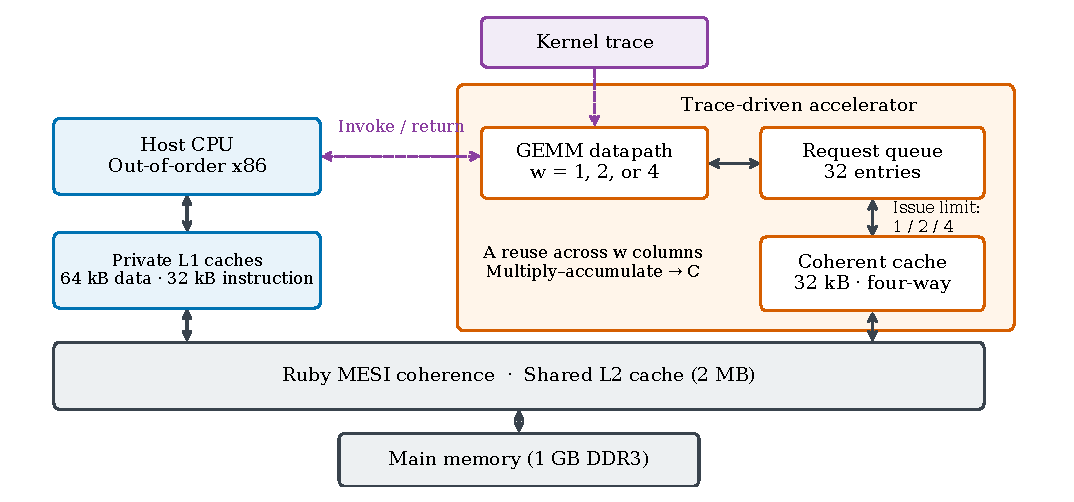
\includegraphics[width=\linewidth]{figures/architecture.pdf}
\caption{Overall simulated architecture. The host invokes the trace-driven GEMM accelerator, whose datapath accesses shared arrays through a bounded request queue and private coherent cache. Solid arrows show bidirectional memory traffic; dashed arrows show invocation and trace inputs. Tile width and request issue limit are the experimental variables.}\label{fig:architecture}
\end{figure*}

Figure~\ref{fig:architecture} shows the system modeled with
gem5-Aladdin~\cite{gem5code,aladdincode}. An out-of-order x86 host and the
accelerator share a Ruby MESI coherent memory system with a 2 MB L2 cache
and 1 GB DDR3 memory. The accelerator replays a kernel dependence graph;
its memory requests pass through a 32-entry queue to a 32 kB, four-way
private cache with 64-byte lines. Each accelerator cycle is 1 ns. We vary
the output-column width and the number of requests allowed per accelerator
cycle while holding the remaining configuration fixed.

\subsection{Datasets and Correctness}
We evaluate $N=8,16,24,32$ and widths 1, 2, and 4 using one fixed simulator
build and configuration. Each experiment uses a freshly generated trace
and freshly compiled CPU and accelerator programs. Their
outputs are checked against the same integer GEMM calculation. A separate
$N=24$ experiment crosses widths 1 and 4 with issue limits 1, 2, and 4,
reusing one trace per kernel. Graph instrumentation and repeated-call
experiments provide additional evidence about memory traffic and cache
history.

\subsection{Timing and Cost}
Offload time runs from accelerator invocation through datapath completion
to host return. We report datapath time separately. Whole-program timing
includes process setup and host work, and CPU speedup compares the CPU and
accelerator execution of the same kernel. Area combines the model's
functional-unit and memory estimates; it is a pre-RTL estimate. The
issue-limit sweep changes request throughput without modeling the physical
area or energy of additional cache ports.

\section{Width, Size, and Modeled Area}
\begin{table}[!t]
\centering
\caption{Main width comparison at $N=24$ and $N=32$. Functional-unit and memory estimates are separate.}
\label{tab:width}
\footnotesize
\setlength{\tabcolsep}{4pt}
\begin{tabular}{rrrrrrr}\toprule
$N$ & $w$ & \shortstack{Datapath\\(ns)} & \shortstack{Offload\\(ns)} & \shortstack{CPU speedup\\($\times$)} & \shortstack{FU area\\(mm$^2$)} & \shortstack{Memory area\\(mm$^2$)} \\ \midrule
24 & 1 & 1452 & 2703 & 1.163 & 0.598 & 0.803 \\
24 & 2 & 1257 & 2508 & 1.163 & 0.598 & 0.803 \\
24 & 4 & 1133 & 2384 & 1.171 & 0.594 & 0.803 \\
32 & 1 & 2827 & 4306 & 1.499 & 0.444 & 0.803 \\
32 & 2 & 2268 & 3508 & 1.491 & 0.793 & 0.803 \\
32 & 4 & 1984 & 3224 & 1.509 & 0.789 & 0.803 \\
\bottomrule
\end{tabular}
\end{table}

\begin{figure*}[!t]\centering
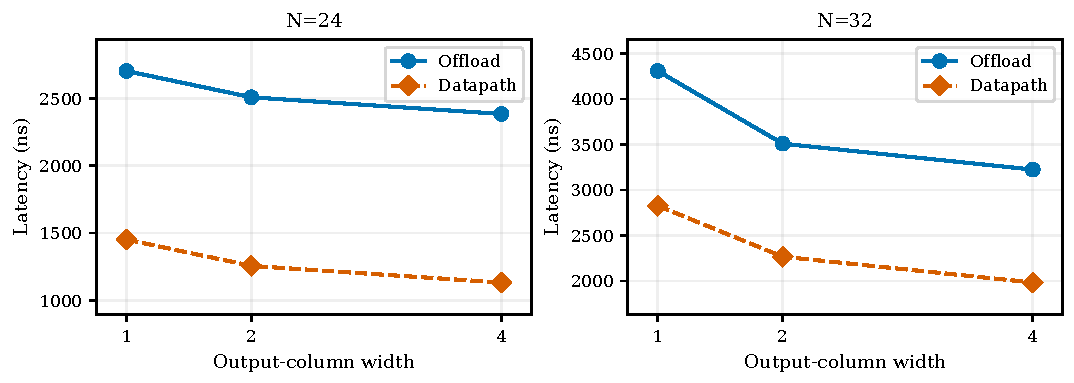
\includegraphics[width=\linewidth]{figures/width_latency.pdf}
\caption{Width versus latency, compared separately at each matrix size.}\label{fig:width}
\end{figure*}

\begin{figure*}[!t]\centering
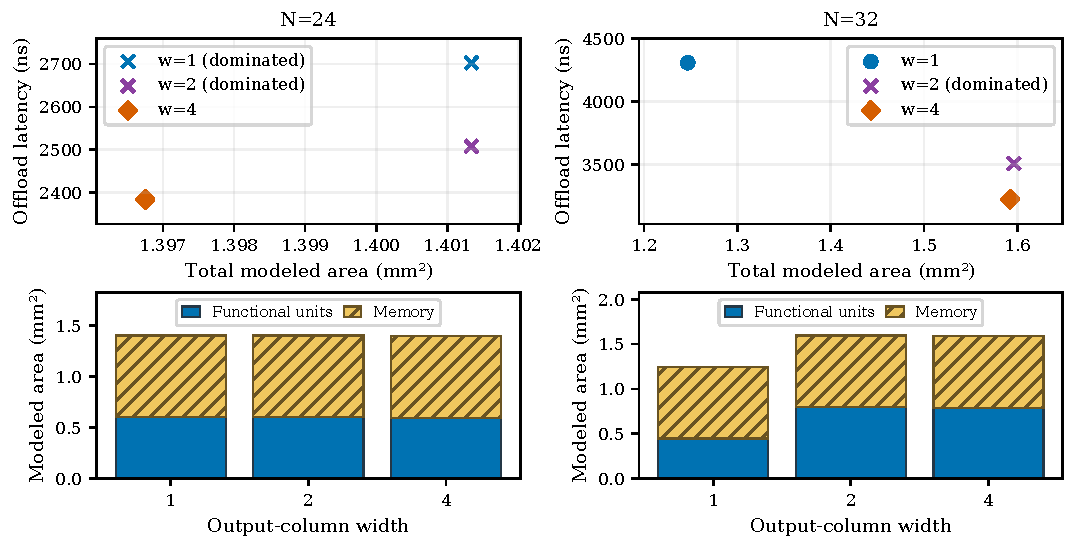
\includegraphics[width=\textwidth]{figures/latency_area.pdf}
\caption{Offload latency versus total modeled area, with functional-unit and memory estimates shown below. Crosses denote dominated points; hatched bars show memory area.}\label{fig:area}
\end{figure*}
\begin{figure}[!t]\centering
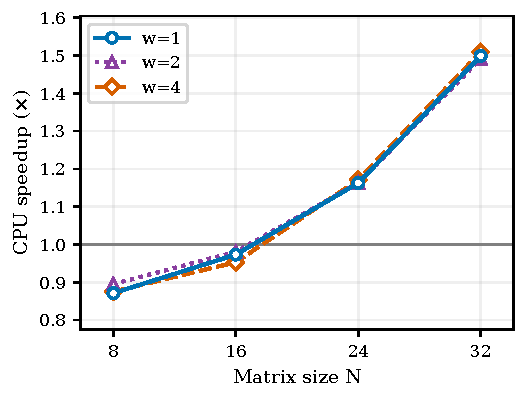
\includegraphics[width=\columnwidth]{figures/cpu_speedup_size.pdf}
\caption{Same-kernel whole-program CPU speedup across all four matrix sizes. Color, line style, and marker distinguish tile widths.}\label{fig:cpu}
\end{figure}

Table~\ref{tab:width} summarizes the main comparisons.
Figure~\ref{fig:width} shows diminishing offload-latency improvements from
increasing width. At $N=24$, width 4 dominates widths 1 and 2 on measured
offload latency and modeled total area. At $N=32$, width 1 and width
4 remain choices: width 1 uses less modeled area, while width 4 is faster.
Width 2 is dominated by width 4. A point is dominated when another width
is no slower and uses no more area, with a strict improvement in at least
one metric. This comparison applies within each matrix size.
Figure~\ref{fig:area} shows these choices and separates functional-unit
and memory estimates.

The same-kernel CPU comparisons in Fig.~\ref{fig:cpu} show that
width 4 is slower than the CPU at $N=8$ (\SpeedupEight$\times$) and
$N=16$ (\SpeedupSixteen$\times$), but faster at $N=24$ (\SpeedupTwentyFour$\times$) and
$N=32$ (\SpeedupThirtyTwo$\times$). Width-4 whole-program
reductions relative to width 1 are \ProgramReductionEight\%, \ProgramReductionSixteen\%, and \ProgramReductionTwentyFour\% at
$N=8,16,24$; the $N=32$ reduction is \ProgramReductionThirtyTwo\%. A local datapath or
offload improvement can therefore be much larger than the application gain.

\section{From Graph Operations to Memory Requests}
To connect source-level reuse to memory traffic, we instrumented the
optimized dependence graph and cache-request interface. Instrumented and
reference runs used the same traces and executables, passed output checks,
and produced matching simulated statistics. This verifies that the observer
does not change the measured behavior.

\begin{table}[!t]
\centering
\caption{Passive diagnostic, $N=24$, issue limit 4. Returned requests equal accepted requests per array.}
\label{tab:graph}
\footnotesize
\setlength{\tabcolsep}{4pt}
\begin{tabular}{rrrrr}\toprule
$w$ & \shortstack{Source $A$\\loads} & \shortstack{Optimized\\$A/B$ loads} & \shortstack{Accepted\\$A/B$ loads} & \shortstack{Accepted\\$C$ stores} \\ \midrule
1 & 13824 & 13824/13824 & 36/36 & 576 \\
2 & 6912 & 6912/13824 & 36/36 & 576 \\
4 & 3456 & 3456/13824 & 36/36 & 576 \\
\bottomrule
\end{tabular}
\end{table}

Table~\ref{tab:graph} connects source and graph operations to accepted requests.
The observer counts connected operations before and after optimization.
It separates GEMM arithmetic contributing to $C$ from address calculations
and control operations. Connected $A$
loads retain the source reduction, while products and accumulation adds
remain \GraphProducts{} and \GraphAdds{}, respectively, for every width.
Nevertheless all three widths accept and return \AcceptedALoads{} $A$
loads, \AcceptedBLoads{} $B$ loads, and \AcceptedCStores{} $C$ stores.

The cache queue merges loads to the same cache line, explaining why fewer
graph loads need not produce fewer accepted requests. Issue-limit blocked
cycles are \IssueBlockedCycles{} for widths 1, 2, and 4. Queue-full blocked
cycles are \QueueBlockedCycles{}. These observations explain unchanged request
traffic and differing scheduling opportunities without establishing one
unique latency bottleneck.

\section{Issue Capacity and Aggregate Cache Evidence}
In the issue-limit experiment (Fig.~\ref{fig:bandwidth}), width-4 offload
reductions relative to the matched width-1 point are \IssueLimitBenefits{}
at issue limits 1, 2, and 4. Across all six points, completion time
exceeds datapath duration by \CompletionResidualNs{} ns and host return
takes \HostReturnNs{} ns: offload time equals datapath time plus
\OffloadResidualUs{} $\mu$s. This is a measured timing offset whose
components have not been causally isolated. At issue limit 4, both widths
reproduce the main $N=24$ experiment's offload times.

\begin{figure*}[!t]\centering
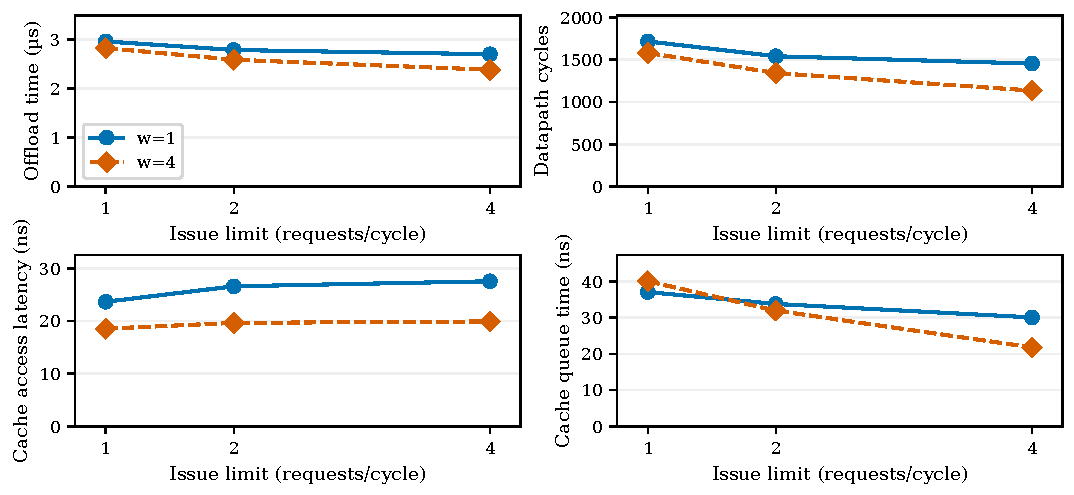
\includegraphics[width=\linewidth]{figures/bandwidth_sensitivity.pdf}
\caption{Issue-limit study at $N=24$, widths 1 and 4, and limits 1, 2, and 4 requests per accelerator cycle. Cache access and queue latencies are means. Cache capacity, queue size, traces, and timing boundaries are fixed.}\label{fig:bandwidth}
\end{figure*}

The L1 protocol increments aggregate demand misses both for absent
lines and for a store upgrade from Shared to Modified. Sequencer aliasing
also means protocol demand actions need not equal datapath responses.
The six $N=24$ points report \DemandMisses{} L1 accelerator demand misses, but
that number does not partition compulsory, capacity, conflict, or coherence
causes. The available aggregate statistics cannot distinguish these
categories. Global Ruby latency histograms also include CPU traffic, and
the queue-time statistic excludes successfully retried requests. These
measurement limits prevent attributing the width benefit to a single
cache-miss mechanism.

\section{Repeated Calls and Replay Limits}
The repeated-call experiment uses $N=24$, three invocations, and widths
1, 2, and 4. Inputs either remain unchanged or follow the same mutations
used to generate the trace. Each case uses the same trace in a harness
that checks every call and a timed harness that checks only the final
output. Timing boundaries and host code are matched across widths.
Full checking between calls reads $A/B/C$ and executes CPU GEMM, changing
the next call's cache/coherence state even though its runtime lies outside
the offload interval.

\begin{table}[!t]
\centering
\caption{Three-call $N=24$ diagnostics. Checker and timed harnesses have different cache histories; full per-call checks pass in the checker runs.}
\label{tab:warm}
\footnotesize
\setlength{\tabcolsep}{4pt}
\begin{tabular}{lrrrr}\toprule
Input & $w$ & \shortstack{Checked cycles\\(calls 0/1/2)} & \shortstack{Timed cycles\\(calls 0/1/2)} & \shortstack{Timed offload (ns)\\(calls 0/1/2)} \\ \midrule
matched & 1 & 1452/624/628 & 1452/246/229 & 3093/772/607 \\
matched & 2 & 1257/666/666 & 1257/246/229 & 2833/772/608 \\
matched & 4 & 1133/683/687 & 1133/246/228 & 2612/772/607 \\
unchanged & 1 & 1452/630/627 & 1452/227/227 & 2681/819/669 \\
unchanged & 2 & 1257/679/679 & 1257/227/227 & 2486/819/669 \\
unchanged & 4 & 1133/696/696 & 1133/246/228 & 2362/838/670 \\
\bottomrule
\end{tabular}
\end{table}

Table~\ref{tab:warm} contrasts per-call correctness and timed histories.
Later invocations are much shorter in the timed harness, while checking
between calls produces a different latency pattern. Checker work, input
mutation, node ordering, and scheduler state all affect this comparison;
the improvement cannot be attributed solely to a warm cache. The unchanged
input case helps separate mutation from repeated-call behavior.

All per-call checks pass when mutations match trace generation, and timed
runs pass a final checksum. This does not independently verify every
intermediate timed output. Mutating inputs independently of the trace
produced incorrect outputs and is excluded from performance comparisons.
The model therefore supports the tested trace-matched inputs, with limited
claims about arbitrary runtime changes.

\section{Reproducibility and Limitations}
The project repository~\cite{artifacts} provides kernels, configurations,
analysis scripts, raw statistics, generated traces, and compiled program
identities for the complete experiment suite. The graph observer is checked
against the reference simulator using identical traces and programs. Every
figure and table is generated from the validated experiment records.

The study covers small deterministic integer GEMM workloads in a
trace-driven model. It does not establish behavior for general inference
workloads or arbitrary runtime inputs. Area estimates remain pre-RTL,
and the issue-limit experiment does not quantify physical cache-port costs.

\section{Conclusion}
Output-column width improves the measured offload interval in the studied
workloads, and a tighter issue interface reduces that benefit. Source and
connected-graph $A$ reuse survives optimization at $N=24$ but does not reduce
accepted cache traffic in the diagnostic experiment. Modeled latency/area
choices differ by workload size, and whole-program benefits are smaller than
local improvements. Aggregate cache statistics and repeated-call data
support these observations while limiting miss-cause and runtime-input
claims. Tile width should therefore be evaluated against workload size,
the memory interface, and whole-program performance together.

\section*{Artifact Availability}
Source, analysis scripts, raw experiment records, and reproduction
instructions are available in the project repository~\cite{artifacts}.

\IEEEtriggeratref{3}
\begin{thebibliography}{5}
\interlinepenalty=10000
\bibitem{aladdin}
Y. S. Shao, B. Reagen, G.-Y. Wei, and D. Brooks,
``Aladdin: A pre-RTL, power-performance accelerator simulator enabling
large design space exploration of customized architectures,''
in \emph{Proc. 41st ACM/IEEE Int. Symp. Computer Architecture (ISCA)}, 2014,
pp. 97--108.
\bibitem{gem5aladdin}
Y. S. Shao, S. L. Xi, V. Srinivasan, G.-Y. Wei, and D. Brooks,
``Co-designing accelerators and SoC interfaces using gem5-Aladdin,''
in \emph{Proc. 49th Annual IEEE/ACM Int. Symp. Microarchitecture (MICRO)},
2016, pp. 1--12.
\bibitem{gem5code}
Harvard Architecture, Circuits and Compilers, ``gem5-Aladdin SoC
simulator,'' source repository. Accessed: Sep. 30, 2026. [Online].
Available: \url{https://github.com/harvard-acc/gem5-aladdin}
\bibitem{aladdincode}
Harvard Architecture, Circuits and Compilers, ``Aladdin: A pre-RTL,
power-performance model for fixed-function accelerators,'' source
repository. Accessed: Sep. 30, 2026. [Online]. Available:
\url{https://github.com/harvard-acc/ALADDIN}
\bibitem{artifacts}
Y. Mahmud, R. M. Ihtemam, and M. Hussain, ``Coherent GEMM accelerator:
Kernels, experiment records, and validation artifacts,'' project
repository, 2026. [Online]. Available:
\url{https://github.com/yasirmahmud/coherent-gemm-accelerator}
\end{thebibliography}
\end{document}
